% Narrative candidate; the approved main_v10_final4.tex and PDF remain frozen.
\documentclass[conference]{IEEEtran}
\usepackage{cite}
\usepackage{amsmath,amssymb}
\usepackage{graphicx,booktabs,placeins,url}
\newif\iffourfigures\fourfigurestrue
\begin{document}
\title{From Connection Loss to Collision: Closed-Loop Fault Assessment of a Fly-Connectome SNN}
\author{\IEEEauthorblockN{Shuchao Gao}
\IEEEauthorblockA{Graduate School of Information, Production and Systems\\
Waseda University\\Tokyo, Japan}}
\maketitle
\bstctlcite{IEEEcontrol}
\begin{abstract}
We assess how connection loss affects collision avoidance in a fly-connectome spiking neural network (SNN). The synthetic pursuit--escape task uses paired deletion masks and two frozen feedback laws. In the baseline receptive-field realization (RF-0), both laws complete all 48 healthy tasks, yet 50\% connection-row deletion yields 37/48 successes under proportional control and 48/48 under relay control. The prespecified secondary relay-minus-proportional net-loss contrast is $-22.9$ percentage points (95\% whole-seed CI $[-33.3,-12.5]$); two independently recalibrated same-prior realizations each yield an uncertain $-4.2$ $[-12.5,0]$. Recalibration, different test cohorts and unequal healthy clearance qualify this comparison. A frozen command-rate warning detects 2/13, 2/3 and 0/1 subsequent collisions in RF-0/A/B. An executable evidence interface checks pairing, timing and task labels, with independent native replay and demonstrated reuse on a delayed tank. Together, these results support task-level assessment for a declared sensing--control realization and fixed 1-s collision horizon.

\end{abstract}
\begin{IEEEkeywords}
spiking neural networks, fault assessment, closed-loop control, reproducibility
\end{IEEEkeywords}
\newcommand{\SystemFigure}{%
\begin{figure*}[t]
\centering
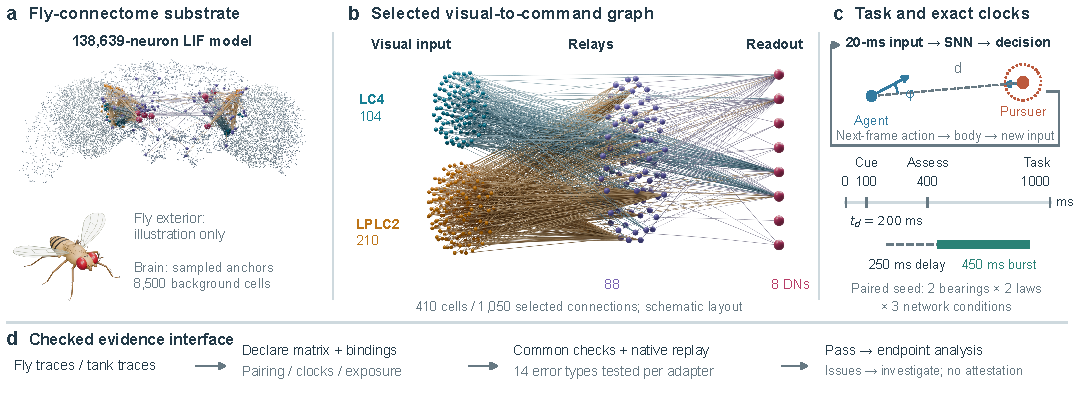
\includegraphics[width=\textwidth]{figs/evidence_v10_overview.pdf}
\caption{System and checked assessment interface. (a,b) Representative model anchors, an illustrative fly and a selected 410-cell/1,050-connection graph. The layout is schematic, not measured neurites or the complete recurrent graph. (c) Sampled feedback and exact burst events; $t_d=200$\,ms is illustrative. (d) Native traces enter common checks and independent replay before endpoint analysis.}
\label{fig:v10f-system}
\end{figure*}}
\newcommand{\ReuseCaption}{Cross-plant reuse and predefined error challenges. (a) First registered tank seed, high inflow, proportional law; level axis is zoomed, safe interval $[0.2,0.8]$. All 96 example tasks remain safe. (b) A requested outflow first changes at 0.60\,s and applies at 0.75\,s, between 100-ms frame boundaries. (c) Eleven common-checker and three native-only cases are detected per adapter, not a general coverage estimate.}
\newcommand{\WarningCaption}{Frozen secondary warning operating points. Rows state contact/success denominators; RF-0/A/B contain 24/12/12 independent seed clusters. Markers show missed-contact and false-alarm rates with pointwise 95\% whole-seed bootstrap CIs. Activity is two-sided; the forecast holds the current command using exact simulated state. Zero observed misses and class-conditional intervals do not establish zero population risk.}
\iffourfigures
\newcommand{\reuseRef}{Fig.~\ref{fig:v10f-reuse}}
\newcommand{\warningRef}{Fig.~\ref{fig:v10f-warning}}
\newcommand{\ReuseFigure}{%
\begin{figure}[t]\centering
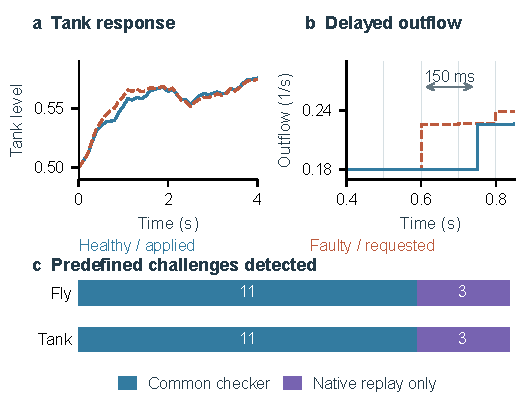
\includegraphics[width=\columnwidth]{figs/v10f_reuse.pdf}
\caption{\ReuseCaption}\label{fig:v10f-reuse}
\end{figure}}
\newcommand{\WarningFigure}{%
\begin{figure}[t]\centering
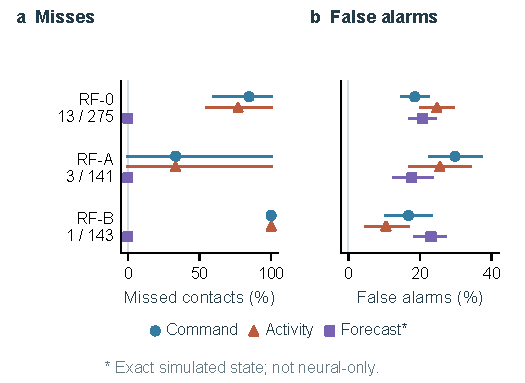
\includegraphics[width=\columnwidth]{figs/v10f_warning.pdf}
\caption{\WarningCaption}\label{fig:v10f-warning}
\end{figure}}
\else
\newcommand{\reuseRef}{Fig.~\ref{fig:v10f-reuse} (left)}
\newcommand{\warningRef}{Fig.~\ref{fig:v10f-warning} (right)}
\newcommand{\ReuseFigure}{%
\begin{figure*}[t]\centering
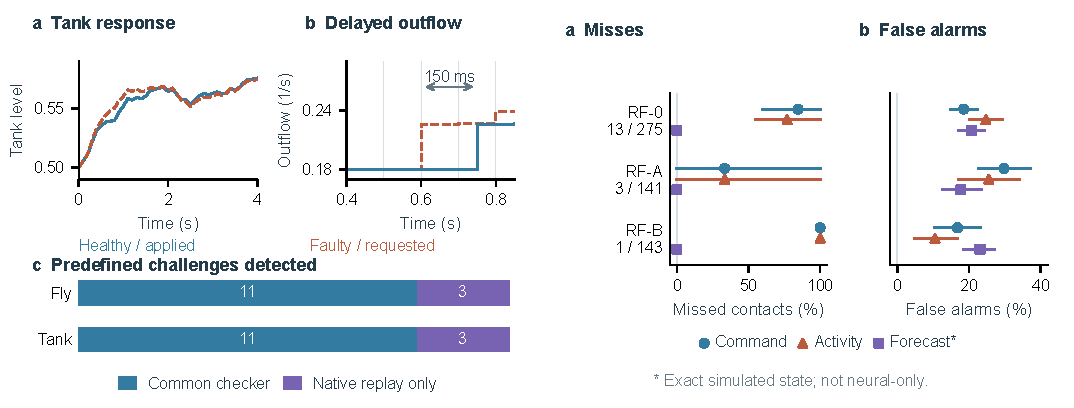
\includegraphics[width=\textwidth]{figs/v10f_reuse_warning.pdf}
\caption{\emph{Left:} \ReuseCaption\ \emph{Right:} \WarningCaption}
\label{fig:v10f-reuse}\label{fig:v10f-warning}
\end{figure*}}
\newcommand{\WarningFigure}{}
\fi
\newcommand{\TransferFigure}{%
\begin{figure*}[t]\centering
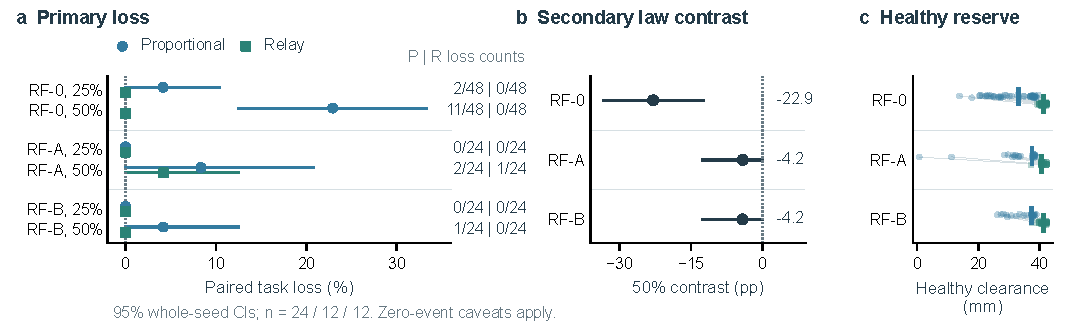
\includegraphics[width=\textwidth]{figs/v10f_rf.pdf}
\caption{Independent RF campaigns. (a) Primary healthy-to-fault losses and P/R loss counts; all healthy tasks succeed and no gains occur. (b) Prespecified secondary relay-minus-proportional net-loss contrast at 50\% deletion, in percentage points. Pointwise 95\% CIs resample whole seeds within each map ($n=24/12/12$), conditional on saved calibrations. (c) All paired healthy minimum-clearance observations, with median bars, show unequal reserve. Maps share a prior but differ in draws, recalibration and test cohorts; differences are not an isolated RF effect.}
\label{fig:v10f-transfer}
\end{figure*}}

\section{Introduction and Positioning}
Can a fly-connectome spiking neural network retain collision avoidance after connection loss? The task outcome depends on the damaged network's interaction with sensing, feedback and delayed actuation. Two control laws can complete the same healthy tasks yet respond differently to matched damage. Assessing this response requires both collision outcomes and executable checks that healthy and damaged runs form the intended pairs over the declared observation horizon.

Connectome-derived models predict sensorimotor outputs\cite{shiu2024drosophila}. An reports task- and state-dependent function preservation under sparsification\cite{an2026sparse}; Jo compares circuit and virtual-arena readouts after connectome damage\cite{jo2026simulating}. Closed-loop fault evaluation is also established: DriveFI searches faults and scenarios that violate autonomous-driving safety constraints\cite{jha2019drivefi}. SpikeFI, SpikingJET and enpheeph provide configurable SNN fault campaigns\cite{spyrou2024spikefi,gogebakan2024spikingjet,colucci2022enpheeph}. These precedents motivate measuring the complete damage-to-task chain, rather than claiming a new fault-injection principle.

CRN synchronization\cite{glasserman1992crn}, hybrid-trajectory monitoring\cite{donze2010breach} and task/resource benchmarking\cite{yik2023neurobench,dangelo2026embodied} supply established tools. Cross-layer NoC analysis connects hardware routing defects to SNN behavior\cite{chessa2026crosslayer}; our functional row deletions supply no comparable physical fault mapping. Here, the evaluated increment is system-level quantification together with executable checks of the evidence supporting it.

We quantify paired task loss under two frozen feedback laws and separately recalibrated, same-prior receptive-field (RF) realizations. We contribute an evidence interface that checks campaign invariants and delegates native input/plant semantics to independent replay, with tested reuse on a delayed tank. We also evaluate frozen neural warnings against later collision, retaining misses, false alarms and uncertain transfer. Together, these contributions connect conditional task outcomes to testable pairing, timing and exposure assumptions.

\SystemFigure
\section{Executable Evidence Contract}
A campaign declares the Cartesian product of seed, condition, law and fault, together with horizon $H$, frame duration and resource units. An adapter normalizes each native record into its condition key, saved-source/map/calibration hashes, input and mask digests, timestamped observations, cumulative resource and first failure. Hashes bind bytes to saved snapshots; they do not attest execution.

The common checker returns an issue code, record key and explanation for incomplete or duplicate matrices, inconsistent bindings, mismatched paired variates/masks, invalid clocks, premature decisions, resource errors and contradictory outcomes. Inputs share variates within seed; each dose shares its mask across laws and bearings. Native replay separately regenerates input events and plant transitions. Feedback-dependent rates and realized events need not match despite shared variates. Warning prefixes expose only observations completed by their stated time, excluding future labels.

\reuseRef\ evaluates the same checker on a distinct tank schema. Its normalized level obeys $\dot h=I-u-0.04h$, initially $h=0.5$, with safe interval $[0.2,0.8]$. Eight seeds cross two nominal inflows (0.15/0.28), two laws and three sensor-sample deletion levels, yielding 96 episodes over 4\,s. Inflow varies uniformly by $\pm0.04$ per frame; measurement noise is uniform over $\pm0.01$. Deleted measurements hold their last value. From measurement $m$, proportional outflow is $\operatorname{clip}(0.18+1.2(m-0.5),0,0.4)$; relay outflow is 0.35 if $m>0.5$, otherwise 0.05. Analytic transitions split at delayed outflow changes, 150\,ms after decisions on a 100-ms grid; generator and replayer use separate algebraic implementations. Resource counts valid sensor updates, not neural spikes.

Each adapter detects eleven predefined cases through common checks and three only through native replay: native-schema, exact-event and geometry/dynamics defects. Real V8 probes independently find six wrong horizon flags, 17 delays of 260 rather than 250\,ms and four completed bursts of 440 rather than 450\,ms. These historical records are excluded from current inference. The challenges are regression evidence, not coverage estimates. A synthetic zero-neural-readout logger passes input/plant checks without neural dynamics, establishing that consistent traces cannot authenticate execution, unlogged neural states or safety.

\ReuseFigure
\TransferFigure
\section{Neural Experiment and Statistical Design}
\subsection{Network, Feedback and Calibration}
The FlyWire v783-derived model\cite{dorkenwald2024neuronal} has 138,639 LIF neurons and 15,091,983 signed, contact-weighted connection rows. We use Shiu parameters\cite{shiu2024drosophila} in Brian~2\cite{stimberg2019brian2}, with 0.1-ms steps, 2.2-ms sensory refractoriness and state/weight restoration before each episode. Assumed Gaussian RFs stimulate 104 LC4 and 210 LPLC2 cells at up to 150\,Hz; other external rates are zero. Eight descending cells provide control features for the timed task (Fig.~\ref{fig:v10f-system}(a--c)).

Between events, $\dot v=(v_0-v+g)/(20\,\mathrm{ms})$ and $\dot g=-g/(5\,\mathrm{ms})$. Threshold $-45$\,mV resets $v$ to $v_0=-52$\,mV and $g$ to zero; both equations pause during refractoriness. Recurrent events add signed contact count times 0.275\,mV to $g$ after 1.8\,ms. External events add 68.75\,mV to voltage. These are functional model parameters, not measured device-fault characteristics.

Input begins at 100\,ms; sensing and feedback update every 20\,ms. Bearing is world-relative angle minus heading; looming is the change of $\arctan(0.05/d)$ at actual separation $d$. The pursuer starts 0.25\,m away at $\pm30^\circ$ and moves at 0.3\,m/s. Each motion segment aims it at the agent's segment-start position. Both positions advance linearly using the agent's starting heading; heading updates at segment end, capped at $\pm100^\circ$. A frame-end decision affects the next frame. The first trigger schedules a 0.35-m/s, heading-fixed burst 250\,ms later for 450\,ms; otherwise speed is 0.05\,m/s. Segments split at exact actuator events; first contact with radius 0.05\,m is solved within each segment. Failure latches, while traces continue to $H=1$\,s for resource accounting. Post-contact activity is counterfactual and excluded from warnings.

For each map, 20 passive development episodes (four seeds, five bearings from $-60^\circ$ to $60^\circ$) fit an affine steering score $z$. Standardized five-frame means of eight command rates over 200--400\,ms predict bearing/$60^\circ$, using ridge penalty 10 and an unpenalized intercept. The trigger threshold is half the tenth percentile of development episode mean command rates over 200--300\,ms, floored at 2.5\,Hz. Before the cue or below threshold, steering is zero. Otherwise proportional/relay laws apply $-600\operatorname{clip}(z,-1,1)$/$-600\operatorname{sgn}(z)$ deg/s outside the burst. Healthy held-out validation RMSE is $65.9^\circ/67.8^\circ/67.2^\circ$ for RF-0/A/B, over eight seed clusters each: $z$ is not an accurate closed-loop bearing estimate.

\subsection{Pairing, Cohorts and Endpoints}
Shared uniforms give nested deletions $w_j^{(f)}=w_j\mathbf1[V_{sj}\geq f]$ and input events $\mathbf1[U_{sk\tau i}<\lambda_{ki}\Delta t]$. Indices denote seed $s$, frame $k$, neural step $\tau$, cell $i$ and connection row $j$; $\Delta t=10^{-4}$\,s. Feedback changes $\lambda$, while input variates and row masks remain paired. Seeds and hashes are traceable, without cross-platform bit-identity guarantees.

RF-0 uses 24 test seed clusters; RF-A/B each use 12 new clusters. Every cluster contains both bearings, two laws and healthy/25\%/50\% deletion: 288/144/144 episodes. New maps independently redraw all 314 azimuths from the same hemisphere prior (left $10$--$90^\circ$, right $-90$--$-10^\circ$), preserving identities, vertical mapping and gradients. Each separately fits the frozen development recipe, uses 32 healthy validation episodes in eight further clusters, then freezes thresholds before testing. All maps, seeds and failures are retained; no test tuning or efficacy stopping occurs. This is transfer with recalibration, not zero-shot transfer or an RF-isolated causal experiment.

With $Y=1$ meaning no contact through $H$, registered primary endpoints are paired loss $L=Y_H(1-Y_F)$, gain $G=(1-Y_H)Y_F$ and activity exposure. Net loss $D=L-G$ is derived. The relay-minus-proportional contrast and warnings are prespecified secondary; trigger-timing and clearance/heading diagnostics are post-hoc. For cumulative spikes $S$ and $T_*=\min(T_F,T_H)$, own-stop and common-duration ratios are
\begin{equation}
R_{\rm stop}=\frac{S_F(T_F)}{S_H(T_H)},\qquad
R_{\rm common}=\frac{S_F(T_*)}{S_H(T_*)}.
\end{equation}
Here $T$ is contact-frame end or $H$, at 20-ms resolution. Common duration remains outcome-dependent and does not equate sensory histories; fixed 400-ms/1-s windows are separate endpoints.

Estimates average both bearings within seed. Pointwise 95\% CIs use 20,000 whole-seed percentile resamples, conditional on stored map/calibration/thresholds (RNG 20261022 for RF-0; 20261023 for transfer). Symmetric-null sign-flip sensitivity tests are Holm-adjusted over two baseline doses, separately from four new map/dose contrasts. Maps and separate angle/action cohorts are not pooled.

Warnings use only data through 400\,ms: unsmoothed 20-ms command rates averaged over 100--400\,ms, or the absolute log spike-count ratio to a law/bearing-specific healthy reference. Each RF's healthy validation separately sets fifth-percentile command/forecast and 95th-percentile two-sided activity cutoffs, frozen before its test cohort; an upper-only comparator flags activity above twice its healthy reference. A held-command forecast uses exact simulated geometry and pending actuation, retaining the current turn; its schedule-only baseline sets future turn to zero. These information-rich forecasts are not neural-only detectors.

\section{Results and Conditional Interpretation}
\subsection{Matched Damage Produces Conditional Task Loss}
Equal healthy success did not imply equal task preservation under matched connection loss (Fig.~\ref{fig:v10f-transfer}). Both laws completed 48/48 healthy RF-0 tasks; at 50\% deletion, P/R succeeded in 37/48 and 48/48. The prespecified secondary relay-minus-proportional net-loss contrast was $-22.9$\,pp (95\% CI $[-33.3,-12.5]$; Holm $p=0.00195$). RF-A/B each yielded $-4.2$\,pp, CI $[-12.5,0]$; all four new map/dose tests have Holm $p=1$. Each new 50\% contrast has only one nonzero cluster. These uncertain contrasts neither precisely reproduce the large baseline advantage nor establish equivalence. The baseline 25\% contrast remains uncertain ($p=0.50$); no 25\% loss is observed in A/B. With twelve event-free clusters, the one-sided 95\% upper bound for any loss in a new identically defined two-bearing cluster is 22.1\%, not zero trial risk.

All four new failures remain: A has P/50\% contacts at seed 3011/$-30^\circ$ and 3009/$+30^\circ$, plus R/50\% at 3009/$+30^\circ$; B has P/50\% at 3110/$-30^\circ$. Healthy reserve differs: RF-0 median P/R minimum clearance is 33.1/41.4\,mm, with absolute heading at 400\,ms of $88.3^\circ/100^\circ$. Thus, the whole-system comparison does not isolate fault-specific tolerance from healthy reserve. Separate map calibrations and test cohorts preclude attributing the smaller contrasts solely to RF changes.

One post-hoc descriptive pair (RF-0 seed 1010, $-30^\circ$, 50\%) shares its mask, 200-ms trigger and 450--900-ms burst schedule, yet P contacts at 964.120\,ms while R remains contact-free through 1\,s. Its healthy P/R clearances already differ (29.2/42.2\,mm). This illustrates the paired outcome, not a protection mechanism. Nine of eleven RF-0 P/50\% contacts occur after 900\,ms; the two transfer law-discordant contacts occur near 995\,ms. The fixed 1-s horizon is therefore part of the result.

\subsection{Neural Warnings Do Not Replace Collision Outcomes}
\WarningFigure
The frozen command warning missed 11/13 RF-0 contacts (\warningRef). It detected 2/3 and 0/1 in A/B, with command false alarms of 51/275, 42/141 and 24/143 successful tasks across RF-0/A/B. The upper-only activity rule detected none. The exact-state held-command forecast detected all observed contacts but flagged 57/275, 25/141 and 33/143 successful tasks. Baseline schedule-only false alarms were 84/275. New sensitivities have only two/one failure clusters; 2,217/7,099 of 20,000 resamples lack a positive class. Intervals omit those draws only for the corresponding conditional rate. Zero-miss empirical intervals do not establish deployable protection.

Own-stop/common-duration medians coincide in all three maps, with maximum paired differences below 0.006. The historical large stopping-time effect does not recur. Fixed windows still differ: P/50\% median 400-ms/1-s ratios are 0.981/1.505, 0.961/1.212 and 0.956/1.139. The separate eight-cluster $\pm45^\circ$ test flags 22/32 healthy activity records and has an uncertain 50\% law contrast. The historical six-cluster 25\% post-hoc $p=0.25$ remains separate, without confirmatory reinterpretation.

\section{Scope, Artifacts and Conclusion}
The neural results describe one graph, an assumed RF family, a synthetic plant, unmatched healthy reserve and sparse failures. Walk-only contact by 0.8\,s follows from this plant's speed construction, not connectome-specific advantage. Functional row deletions establish no biological tolerance, physical upset rate, hardware safety, energy or area benefit. The interface makes declared pairing, timing and exposure testable across two native schemas; it does not prove arbitrary fault coverage or authentic neural execution.

The fixed V10 code/data snapshot\cite{artifactV10} provides both adapters, 576 neural test records, 96 tank examples, frozen configurations and a minimal replay entry point. Original generation-time versions are preserved. Saved-data replay requires no external matrices; fresh neural simulation requires separately obtained, hash-matched inputs. Third-party tables with unresolved redistribution terms are excluded. A fresh checkout and clean dependency installation previously reproduced 448 V9 saved traces on the same host, without establishing second-host neural replication. New RF tests used four Xeon W-2223 workers, about 179\,s median episode wall time and at most 1.21\,GiB lifetime working set per worker.

Paired connection loss produced different collision outcomes despite equal healthy success. Smaller, uncertain contrasts in separately recalibrated RF realizations and the observed warning errors qualify the baseline finding. Executable pairing checks and independent native replay make these conditional results auditable, with limited reuse beyond the fly task. This task-level assessment provides a basis for evaluating how future device-level nonidealities propagate through neuromorphic controllers to closed-loop behavior.

\FloatBarrier\clearpage
\bibliographystyle{IEEEtran}
\bibliography{refs}
\end{document}
